\chapter{Visualisierung der Greenschen Funktion}
\rhead{Visualisierung der Greenschen Funktion}
\begin{refsection}
\chapterauthor{Andreas Linggi, Stefan Steiner}

\section{Aufgabenstellung}

Um ein Problem der Mathematik besser zu verstehen, ist es oft sehr
hilfreich, wenn es verst"andlich beschrieben ist. Eine Visualisierung
in Form eines Bildes oder kurzen Films ist dabei eine M"oglichkeit,
dies zu bewerkstelligen.
	
Ziel dieses Projektes war, die Greensche Funktion in zwei Dimensionen
zu visualisieren. Die L"osung f"ur eine Dimension wurde bereits in
einem kurzen Film veranschaulicht
\footnote{\url{https://www.youtube.com/watch?v=Wpi7Gf7V2HY}}. Es
soll dabei zuerst eine partielle Differentialgleichung gel"ost und
danach visualisiert werden. Die Greensche Funktion erm"oglicht die
Berechnung eines Problems durch Superposition. Darum sollten auch
verschiedene Anfangswerte untersucht werden und wie diese sich auf
die L"osungen auswirken.
	
Als Differentialgleichung ist das Potentialproblem vorgegeben.
Gegeben ist eine leitende Platte, die am Rande geerdet sei. Wenn
nun ein Potential an einem oder mehreren Punkten auf dieser Platte
anliegt, ist es von Interesse zu wissen, welches Potential man nun
an einem beliebigen Punkt auf der Platte misst.

\section{George Green}

Der Namensgeber f"ur die Greensche Funktion ist George Green. Er
war ein britischer Physiker und Mathematiker. Geboren wurde er 1793
in der N"ahe von Nottingham. Sein Vater betrieb eine M"uhle und
George Green arbeitete ebenfalls als M"uller. Nach dem Tod seines
Vaters f"uhrte er den M"uhlenbetrieb fort. Bemerkenswert ist, dass
Green nur etwa zwei Jahre in die Schule ging. Mathematische und
Physikalische Grundlagen brachte er sich selber bei. Der Ort an dem
er lernte war seine M"uhle. Da nie ein Portrait von ihm angefertigt
wurde, gibt es kein Bild von ihm. Darum wird anstatt seinem Konterfei
jeweils eine Windm"uhle verwendet um ihn darzustellen. Die Windm"uhle
gibt es "ubrigens immer noch. Green ver"offentliche mit etwa dreissig
Jahren seine erste Arbeit. Diese wurde kaum beachtet, ausser von
einem adligen Mathematiker namens Sir Edward Bromhead. Er ermutigte
Green, im Alter von vierzig Jahren, in Cambridge zu studieren.
Interessant zu wissen ist dazu, dass dort zu dieser Zeit die Theorien
von Laplace und Fourier noch nicht gelehrt wurden. Green hatte sich
jedoch durch diese Theorien gelesen und sogar noch einige Erweiterungen
hinzugef"ugt. Vier Jahre nachdem er graduierte und kurz vor seinem
internationalen Durchbruch stand, starb er 1841 jedoch an einer
schweren Grippe. Dadurch geriet seine Arbeit f"ur einige Zeit in
Vergessenheit.
	
George Green ist besonders bekannt f"ur das Greensche Theorem und
die Greensche Funktion. Er besch"aftigte sich mit der L"osung von
partiellen Differentialgleichungen und stellte damit unter anderem
mathematische Hilfsmittel bereit, die sogar in der Quantenfeldtheorie
im 20. Jahrhundert von Bedeutung waren \cite{wiki:green}.
	
Neben vielen anderen Pers"onlichkeiten wie Maxwell, Dirac oder
Newton ist er in der Westminster Abbey in London mit einer Gedenktafel
verewigt \cite{wiki:westminster}. Der Grund, warum George Green nicht
so popul"ar ist wie Gauss oder Maxwell, liegt wahrscheinlich darin,
dass von seiner Zeit, als er in seiner M"uhle gearbeitet hat, wenig
bekannt ist. Auch war er nur f"ur sehr kurze Zeit in Cambridge
t"atig.

\begin{figure}                    
\centering 
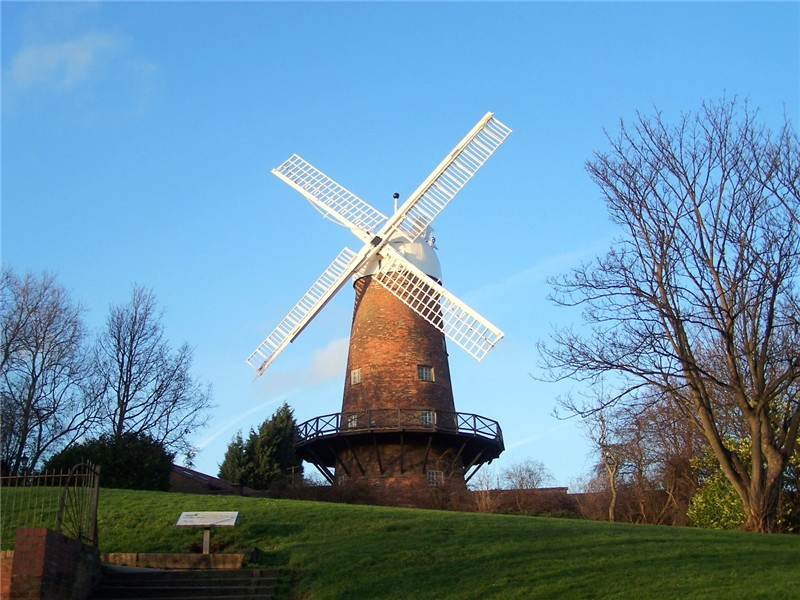
\includegraphics[width=\hsize]{green/images/greens_windmill.jpg} 
\caption{Windm"uhle, in der Green f"ur lange Zeit gearbeitet hat} 
\label{fig:abb1} 
\end{figure} 
	
\section{Algorithmus}
Um eine Visualisierung "uberhaupt durchf"uhren zu k"onnen, braucht
es in unserem Fall Daten, mit denen wir arbeiten k"onnen. Diese
liefert uns ein Programm, bei welchem wir Daten einspeisen und im
Gegenzug bearbeitet erhalten.
	
Das Problem, welches wir hier l"osen, wurde ebenfalls von Philip
Solenthaler und Reto Christen bearbeitet. Sie haben untersucht, wie
ein Programm geschrieben werden kann, welches dieses Problem
m"oglichst effizient l"ost.

\subsection{Mathematischer Ansatz zur L"osung}

Das Potentialproblem auf der leitenden Platte, welches wir l"osen
m"ochten, hat nun folgende partielle Differentialgleichung:
\begin{equation}\label{eq:gleichung}
\dfrac{\partial^2 u}{\partial x^2}+\dfrac{\partial^2 u}{\partial y^2} = f(x,y).
\end{equation}
Wobei die Rand-, und Anfangsbedingungen auf der leitenden Platte alle null sind. 
	
Die quadratische Platte mit der L"ange $n\times n$ wird dabei mit
den Werten $u_{ij}$ diskretisiert, wobei $0 < i,j<n$. Wir bekommen
eine endliche Anzahl an Werte $u$.
%	 Dabei wird f"ur jeden Wert $u$ diese Gleichung gel"ost. 
Der Ansatz f"ur eine L"osung dieses Problems bietet die lineare
Algebra, welcher bereits im Theorieteil des Skriptes ausf"uhrlich
hergeleitet wird. Das bedeutet, wir m"ussen ein Problem folgender
Art l"osen.
\begin{equation}
Au = f
\end{equation}
Es sei dabei $A$ die Koeffizientenmatrix, $f$ der St"orvektor und
$u$ der L"osungsvektor.
	
Die leitende Platte wird als eine Fl"ache visualisiert. Um diese
als Vektor $u$ zu schreiben ist dabei festgelegt worden, dass die
Spalten dieser diskretisierten Fl"ache untereinander geschrieben
werden. Dies ergibt Vektoren der l"ange $n^2$.
	
Aus diesem Zusammenhang heraus ergibt sich dabei die Koeffizientenmatrix
$A$.
\[
	A=\left(
	\begin{array}{ccccc|ccccc|c|ccccc}
	    -4&     1&     0&\cdots&     0 &     1&     0&     0&\cdots&     0 &\cdots &      &      &      &      &      \\
	     1&    -4&     1&\cdots&     0 &     0&     1&     0&\cdots&     0 &\cdots &      &      &      &      &      \\
	     0&     1&    -4&\cdots&     0 &     0&     0&     1&\cdots&     0 &\cdots &      &      &     0&      &      \\
	\vdots&\vdots&\vdots&\ddots&\vdots &\vdots&\vdots&\vdots&\ddots&\vdots &       &      &      &      &      &      \\
	     0&     0&     0&\cdots&    -4 &     0&     0&     0&\dots &     1 &\cdots &      &      &      &      &      \\
	\hline
	     1&     0&     0&\cdots&     0 &    -4&     1&     0&\dots &     0 &\cdots &      &      &      &      &      \\
	     0&     1&     0&\cdots&     0 &     1&    -4&     1&\dots &     0 &\cdots &      &      &      &      &      \\
	     0&     0&     1&\cdots&     0 &     0&     1&    -4&\dots &     0 &\cdots &      &      &     0&      &      \\
	\vdots&\vdots&\vdots&\ddots&\vdots &\vdots&\vdots&\vdots&\ddots&\vdots &       &      &      &      &      &      \\
	     0&     0&     0&\cdots&     1 &     0&     0&     0&\cdots&    -4 &\cdots &      &      &      &      &      \\
	\hline
	\vdots&\vdots&\vdots&      &\vdots &\vdots&\vdots&\vdots&      &\vdots &\ddots &\vdots&\vdots&\vdots&      &\vdots\\
	\hline
	      &      &      &      &       &      &      &      &      &       &\cdots &    -4&     1&     0&\cdots&     0\\
	      &      &      &      &       &      &      &      &      &       &\cdots &     1&    -4&     1&\cdots&     0\\
	      &      &     0&      &       &      &      &     0&      &       &\cdots &     0&     1&    -4&\cdots&     0\\
	      &      &      &      &       &      &      &      &      &       &       &\vdots&\vdots&\vdots&\ddots&\vdots\\
	      &      &      &      &       &      &      &      &      &       &\cdots &     0&     0&     0&\cdots&    -4\\
	\end{array}
	\right) 
	\]

\subsection{Technische Umsetzung}

Die Matrix $A$ enth"alt die Koeffizienten f"ur die partielle
Differentialgleichung der zweiten Ordnung. Sie hat die Gr"osse $n^2
\times n^2$. Diese Matrix im Arbeitsspeicher abzuspeichern w"are
f"ur mittelgrosse Matrizen schon nicht mehr
m"oglich \cite{mueller:hpcseminar}.
	
Der ben"otigte Speicher f"ur eine Platte mit der Gr"osse $500 \times
500$ und \verb|float| Werten (4 Byte) w"are
	
\begin{equation}
500^2 \times 500^2 \cdot 4\;\mathrm{Byte} = 232.8\;\mathrm{GByte}
\end{equation}
	
Mit $n = 1000$ sogar 3.64\,TByte, also definitiv zu viel. Dies ist
aber auch gar nicht n"otig. Es m"ussen jeweils nur die Nachbarelemente
von $u_{ij}$ addiert und durch einen konstanten Faktor geteilt
werden, die Randelemente sind dabei Null zu setzen.

\begin{eqnarray}
%		f_{ij} = u_{i-i,j}+u_{i+1,j}+u_{i,j+1}+u_{i,j-1}-4u_{ij}\\
u_{ij} = \dfrac{u_{i-i,j}+u_{i+1,j}+u_{i,j+1}+u_{i,j-1}-f_{ij}}{4}
\label{eq:gauss-seidel}
\end{eqnarray}
	
Da die diskretisierte partielle Ableitung jeweils nur die Elemente
ober/unterhalb und links/rechts des aktuellen Elementes in die
Rechnung mit einbezieht (\ref{eq:gauss-seidel}), m"ussen mindestens
$n$ Iterationen durchgef"uhrt werden, damit sich das Potential "uber
die ganze Ebene verteilt.
	
\subsubsection{Parallelisierung}
	
Um das Gleichungssystem (\ref{eq:gleichung}) zu l"osen, haben wir
den Gauss-Seidel Algorithmus benutzt. Bei diesem Algorithmus ist
die aktuelle Zeile von der vorherigen abh"angig. Bei der Parallelisierung
wird das Gleichungssystem an verschiedenen Stellen zu l"osen begonnen.
Das ist zwar nicht so effizient, wie ein "'normaler"' Gauss-Seidel,
wird aber durch die Parallelisierung schneller.
		
Die Abweichung ist bei den ersten Schritten am gr"ossten, und wird
bei jeder Iteration kleiner. Als wir die ersten Berechnungen durch
gef"uhrt hatten, fiel uns auf, dass die einzelnen Threads am Anfang
gut als Linien von Spitzen sichtbar sind (\ref{fig:201_1}).
		
\begin{figure}
\centering
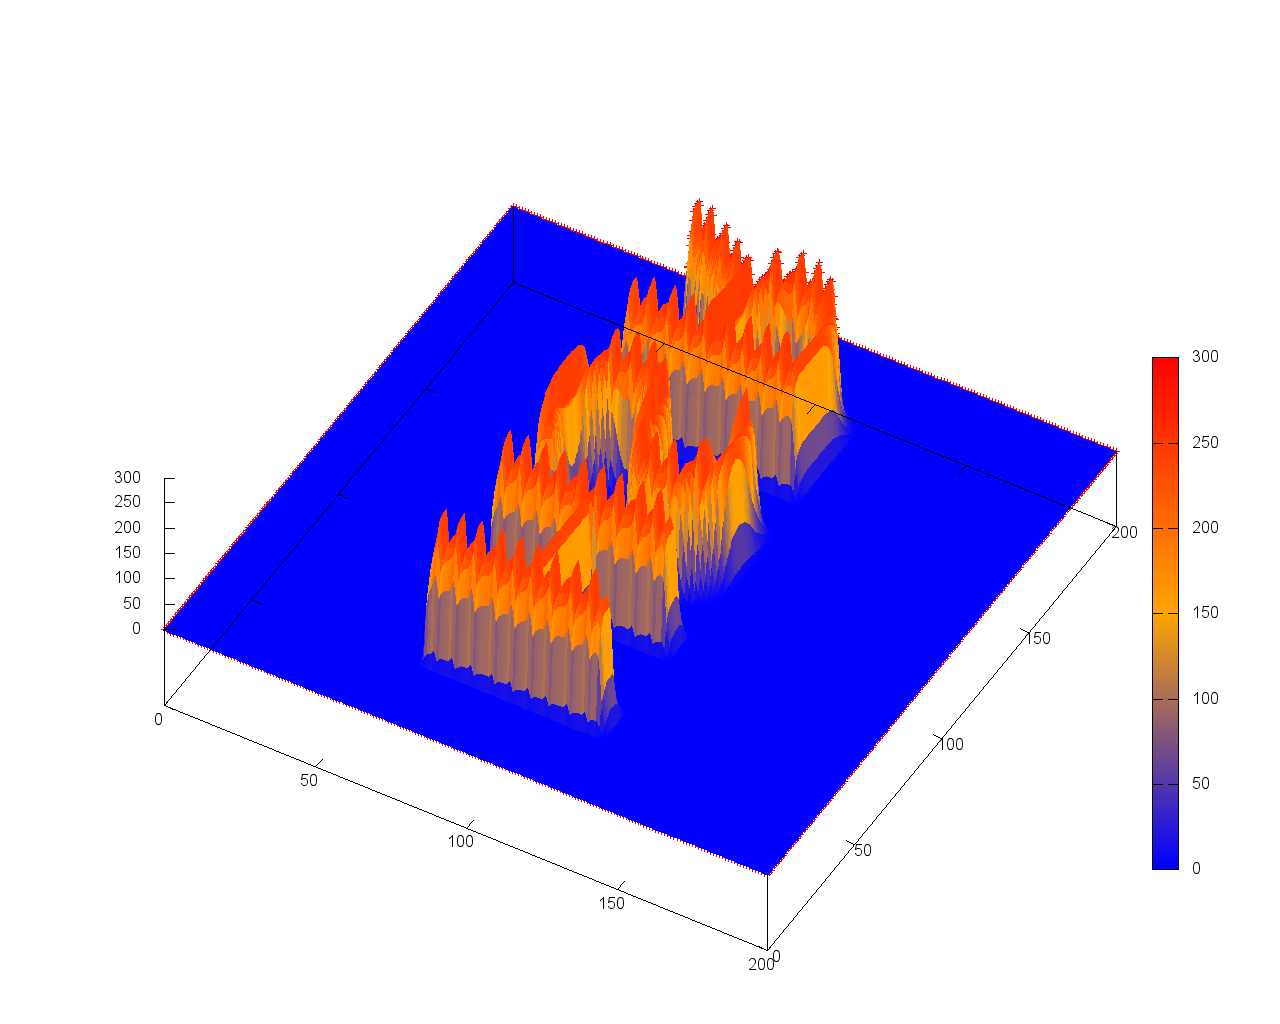
\includegraphics[width=\hsize]{green/images/step001}
\caption{Berechnung von einer $201 \times 201$ Fl"ache mit 32 Threads
nach dem ersten Iterationsschritt}
\label{fig:201_1}
\end{figure}
		
		
Wir haben uns f"ur Open-MP entschieden, da es f"ur uns die einfachste
Methode war, die Berechnung zu parallelisieren. Wie bei der Arbeit
von Christen und Solenthaler erkl"art, w"are Open-MPI die effizienteste
Weise, um solch ein Problem zu l"osen. Da hier nur die Resultate
des Algorithmus von Interesse waren und wir relativ kleine Probleme
gel"ost haben, hat es sich nicht gelohnt, den Mehraufwand f"ur
Open-MPI zu betreiben. Die Rechenzeit war absolut im Rahmen.
		
Wie schon beim Kugelsternhaufen erw"ahnt, ist nun diese Open-MP
Parallelisierung einfach zu realisieren, wie folgendes Beispiel
zeigt.
		
\begin{code}
// Parallelisierung einer for-Schleife
	int numthreads = 32;
	#pragma omp parallel for num_threads(numthreads)
		for (i = 0; i < dim; i++)
		{ ...
\end{code}

\subsubsection{Dateiformate}
	
Um mit der Datenflut umgehen zu k"onnen, musste ebenfalls eine
L"osung entwickelt werden. Als Eingabedatei wurde ein Bild im FITS
Format verwendet. Da es jedoch einfacher schien, wurde w"ahrend des
Programmes mit \texttt{.csv} Files gearbeitet. Dabei war der
technische Aufwand gering und die Resultate konnten schnell
kontrolliert werden. Aus diesen \texttt{.csv} Dateien kann mit GNU-Plot ein
Bild erstellt werden. Optional dienen diese als Vorlage f"ur einen
kurzen Film.

\section{Visualisierung}
	
\subsection{Prinzip}
			
Ziel der Visualisierung ist, die einzelnen Schritte einer Berechnung
mit der Greenschen Funktion zu zeigen. Bei jedem Schritt kommen
zus"atzliche Werte zum vorherigen Schritt hinzu. Die Bilder aus
\ref{fig:dreiSchritte} stellen drei solche Schritte dar, wie wir
sie in unserer Arbeit definiert haben.
		
W"urden wir jeweils die L"osungen f"ur alle Werte $u_{ij}$ einzeln
berechnen und sie dann addieren, m"ussten wir diese Schritte
schlussendlich noch visuell darstellen. Der Aufwand hierf"ur ist
aber betr"achtlich. Da die Darstellung im Vordergrund steht, ist das Verfahren zur
Berechnung irrelevant f"ur das Endergebnis. Um die Rechnung zu
beschleunigen, haben wir uns f"ur einen anderen Algorithmus
entschieden, welcher uns erlaubt, so viele Werte $u_{ij}$ wie n"otig
miteinander zu l"osen.
		
Wir werden dementsprechend immer das gleiche Problem l"osen mit
jeweils zus"atzlichen Werten $u$. Jeder dieser Schritte hat ein
Bild mit den vorherigen plus den neuen Werten zur Folge. Zusammengestellt
ergeben diese Bilder eine anschauliche Visualisierung der Greenschen
Funktion.
	
	
\subsection{Darstellungsm"oglichkeiten}
	
Welche Werte wir jeweils in einem Schritt dazu nehmen ist noch
offen. Man k"onnte beispielsweise die Fl"ache von oben links bis
unten rechts durchgehen und immer ein oder mehrere Punkte dazu
nehmen. Es ist auch vorstellbar, diese Punkte zuf"allig auszuw"ahlen,
bis alle Punkte berechnet wurden. Der Nachteil dieser Verfahren
ist, dass sie nicht viel weniger aufw"andig sind, als das Verfahren,
welches alle Punkte einzeln berechnet. Wenn beispielsweise eine
Fl"ache bzw. Bild mit $500 \times 500$ Werten berechnet werden soll,
muss das Problem 250\,000 mal vollst"andig gel"ost werden. Es w"aren
auch 250\,000 Bilder vorhanden, eine Datenflut, die unser Auge wohl
kaum bew"altigen kann. Es ist fraglich, wie sinnvoll eine solche
Visualisierung ist.
		
Um das zu verhindern, haben wir uns entschieden, in der Mitte einer
solchen Fl"ache zu beginnen und dann schrittweise, Ring f"ur Ring,
nach aussen zugehen.

\begin{figure}
\centering
\begin{tabular}{ccc}
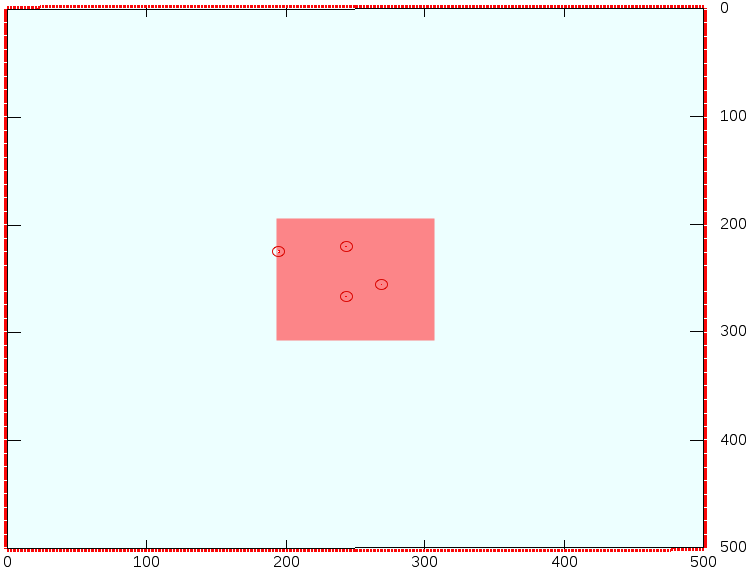
\includegraphics[width=0.3\hsize]{green/images/resultate/grfl/step0057.png}
& 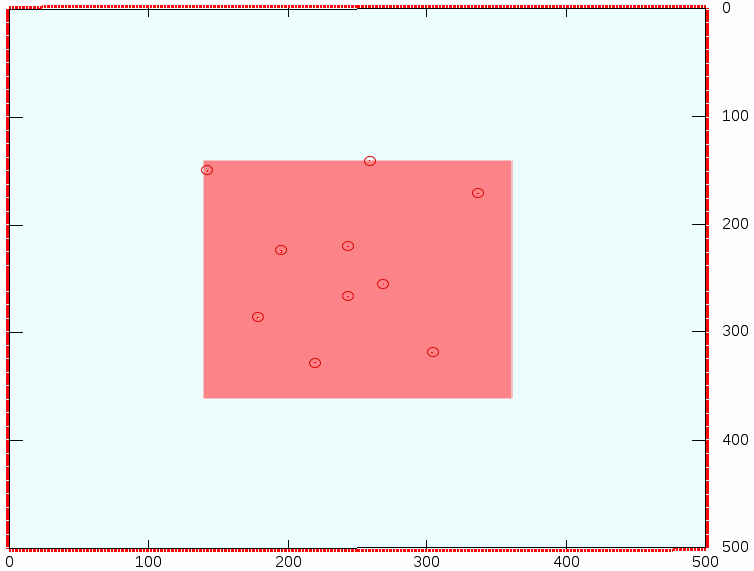
\includegraphics[width=0.3\hsize]{green/images/resultate/grfl/step0111.png}
& 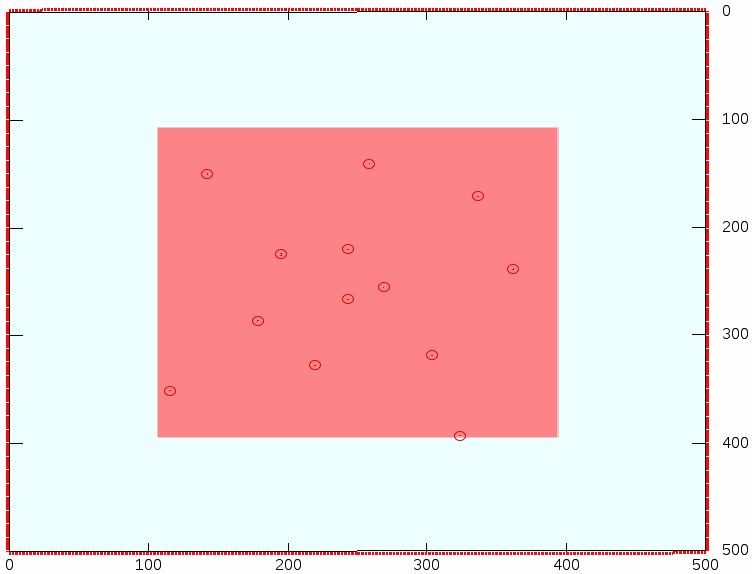
\includegraphics[width=0.3\hsize]{green/images/resultate/grfl/step0144.png}
\end{tabular}		
\caption{Die Schritte 57, 111 und 144 auf einer Fl"ache, die durch
$500 \times 500$ Werte dargestellt wird.}
\label{fig:dreiSchritte}
\end{figure}
	
In jedem dieser drei Schritte werden nur die roten Punkte in die
Berechnung ber"ucksichtigt, die anderen werden gleich Null gesetzt.
Jeder Schritt wird vollst"andig gel"ost, bis der maximale Fehler
eine Grenze unterschreitet.
	
\subsection{Technische Umsetzung}
	
Vor jeder dieser Berechnungen wird ein Vektor $f$, der unsere Fl"ache
repr"asentiert, so manipuliert, dass der helle "aussere Bereich
gleich Null gesetzt wird. Danach wird die Berechnung, die in jedem
Schritt identisch ist, durchgef"uhrt.
		
Wir speichern den berechneten Vektor $u$ als Matrix in einem \texttt{.csv}
File mit einer Genauigkeit von vier Nachkommastellen ab, was f"ur
eine Visualisierung gen"ugt. Anfangs benutzten wir MATLAB um aus
dem \texttt{.csv}-File eine anst"andige Visualisierung zu erhalten. Der
Aufwand war gering und die Resultate waren schnell kontrollierbar.
		
\lstinputlisting{green/csvToMatrixAndPlot.m}
		
Um das zu automatisieren benutzen wir sp"ater Gnuplot, welches sich
mit C-Code ohne Probleme ansprechen l"asst und uns die Bilder
automatisch mit dem vorgegebenen Einstellungen erstellt.
		
fmt: standard input: Illegal byte sequence
Gnuplot ist ein Kommandozeilen basiertes OpenSource Tool, das aber
auch mit GUI erh"altlich ist.
		
\lstinputlisting{green/gnuplot.c}
	
\subsection{Generieren der Bilder}
	
Die Bilder werden, nachdem alle Einzelschritte berechnet wurden, aus
den Dateien wiederum parallelisiert in einer \verb|for|-Schleife
zu \texttt{.png} Bilddateien verarbeitet. Da der letzte Schritt das Maximum
bzw. Minimum aller Schritte enth"alt, sofern wir nur Potentiale mit
gleichen Vorzeichen haben, wird die Skalierung der $z$-Achse direkt
aus diesen Daten berechnet. Dies garantiert und eine optimale
Darstellung.
		
Wir haben jeweils zwei verschiedene Ansichten erstellt: Eine normal
Ansicht, d.h ein 3D-Plot wie er z.~B.~in \ref{fig:201_1} zusehen
ist und eine Ansicht von oben mit H"ohenlinien. Aus den Bilddateien
wird am Schluss optional noch ein Video erstellt.
		
\section{Probleme}

\subsection{Konvergenz}
	
Wir haben anfangs den HSR-Schriftzug als FITS-File in eine Matrix 
eingelesen und diesen als Vektor $f$ abgespeichert. Der maximale
Wert des L"osungsvektors $u$ betrug anfangs nur 255, stieg nach
einigen hundert Iterationen auf "uber 3000 an und die Funktion nahm
die Form eines Haufens an. Wir hatten mit einem anderem Resultat
gerechnet und "uberpr"uften unseren Algorithmus. Wir entdeckten
keinen Fehler in unserem Algorithmus und konnten die Werte mit
MATLAB verifizieren. Die n"achste Frage war, ob der Gauss-Seidel
Algorithmus konvergiert. Wir berechneten den Spektralradius der
Matrix $A$ gem"ass Definition\;5.1 aus dem Skript
HPC\cite{mueller:hpcseminar}:
	
\begin{eqnarray}
A = M+N\\
\varrho(M^{-1}N)<1
\end{eqnarray}
		
Die Gr"osse der Matrix $A$ nimmt mit $n^4$ zu, weshalb die Berechnung
der Spektralradien mit MATLAB sehr schnell rechenaufw"andig wird.
Darum haben wir nur Spektralradien mit kleinem $n$ berechnet.
		
\begin{table}
\begin{tabular}{cc}
n & Specktralradius $\varrho$\\\hline
5 & 0.7500\\
10 & 0.92063\\
15 & 0.96194\\
20 & 0.97779\\
25 & 0.98547\\
40 & 0.99414
\end{tabular}
\centering
\caption{Spaktralradien der Matrix $A$ f"ur eine Matrix $f$ mit der Gr"osse $n\times n$}
\end{table}
	
Einerseits sind alle Spaktralradien kleiner Eins, was gut ist,
andererseits sind sie sehr nahe bei Eins, was erkl"art wieso unser
Algorithmus so langsam konvergiert.
		
Wir hatten sp"ater Erfolge, wenn wir die Anfangswerte des Vektors
$f$ klein w"ahlten $(f_{ij}<1)$. So waren die Fehler von Anfang an
kleiner und wir bekamen brauchbare Werte.
	
\subsection{Datenflut}
	
Bei Platten mit feiner Diskreditierung mussten wir darauf achten,
dass wir nicht zu viele Daten abspeichern. Wir mussten das Programm
so umschreiben, dass wir einstellen konnten, wie viele Bilder wir
schlussendlich wollten. Anhand dieser Einstellung wurden nur
die ben"otigten \texttt{.csv} und \texttt{.png} Dateien abgespeichert.
Das Programm wurde dadurch automatisch auch gleich viel schneller.
		
\begin{beispiel}
Wir wollen eine Platte mit  $40 \times 40$ Werten berechnen. Um die
Konvergenz beobachten zu k"onnen, speichern wir nach jeder Iteration
die Werte in eine \texttt{.csv} Datei ab. Es sind etwa 3000 bis 4000 Iterationen
n"otig bis sich die Werte nicht mehr ver"andern. Das ist problemlos m"oglich.
			
Wir wollen mehr, eine Platte mit $500 \times 500$ Werten. Um hier
eine Konvergenz zu beobachten, sind etwa 160\,000 bis 180\,000
Iterationen n"otig, wie wir sp"ater herausgefunden haben. Das Ganze
ist nat"urlich stark vom Ausgangsbild abh"angig.

Eine \texttt{.csv} Datei ist dann etwa 1.8\,MB gross, d.~h.~wir wollen ca.~300\,GB
abspeichern. Dies ist m"oglich, sofern gen"ugen Platz vorhanden
ist. Das eigentliche  Problem ist aber, dass das Programm nur noch
mit Daten speichern besch"aftigt ist und kaum noch Zeit zum Rechnen
hat.
\end{beispiel}
	
\subsection{Geeigneter Vektor $f$ finden}\label{sec:geeignetesF}

Ein ganz anderes Problem war, ein geeignetes Bild f"ur die Platte zu finden.
Es sollte die "Uberlagerung der Werte gut zeigen. Wir versuchten
verschiedene Muster, von einem Schriftzug, einzelne Buchstaben bis
zu einzelnen Punkten. Bew"ahrt hat sich eine Spirale. Da wir von
innen nach aussen gehen, kommen immer wieder neue Werte an verschiedenen
Seiten hinzu. Da schlussendlich nur eine geringe Anzahl Punkte
vorhanden sind, wirkt die Visualisierung nicht "uberladen und ist
"ubersichtlich.
		
\section{Resultate}

Wir haben mehrere Platten mit unterschiedlichen Potentialverteilungen
und mit unterschiedlicher Anzahl Diskretisierungspunkten berechnet.
Je nach Ausgangsbild, welches unsere Potentialverteilung darstellt,
ist die Superposition mehr oder weniger gut erkennbar. Wie in
\ref{sec:geeignetesF} erw"ahnt, hat sich eine Spirale von Punkten
bew"ahrt, die wir hier anhand vier verschiedenen Schritten zeigen
wollen. Das erste Bild ist jeweils die Fl"ache f"ur den jeweiligen
Schritt. Alle Punkte haben das selbe Potential. Pro Bild f"uhrten
wir 180\,000 Iterationen durch.

\newlength\breite
\begin{figure}
\centering
\begin{tabular}{cc}
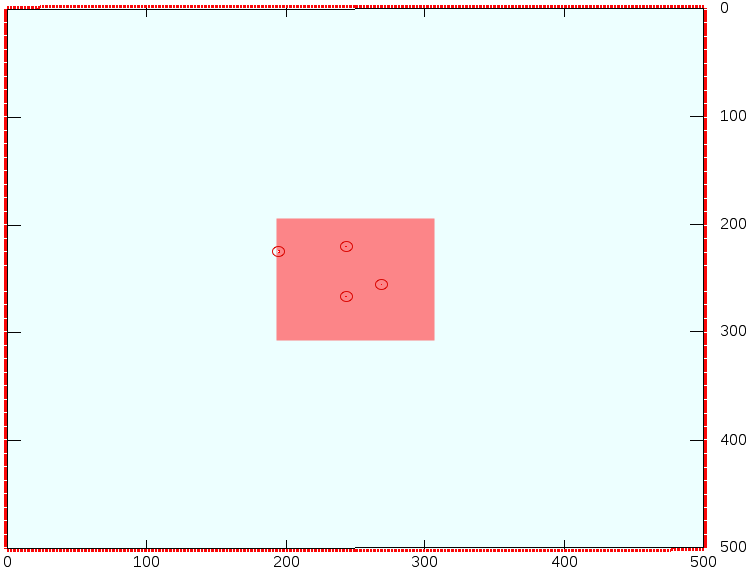
\includegraphics[width=0.48\hsize]{green/images/resultate/grfl/step0057.png}
& 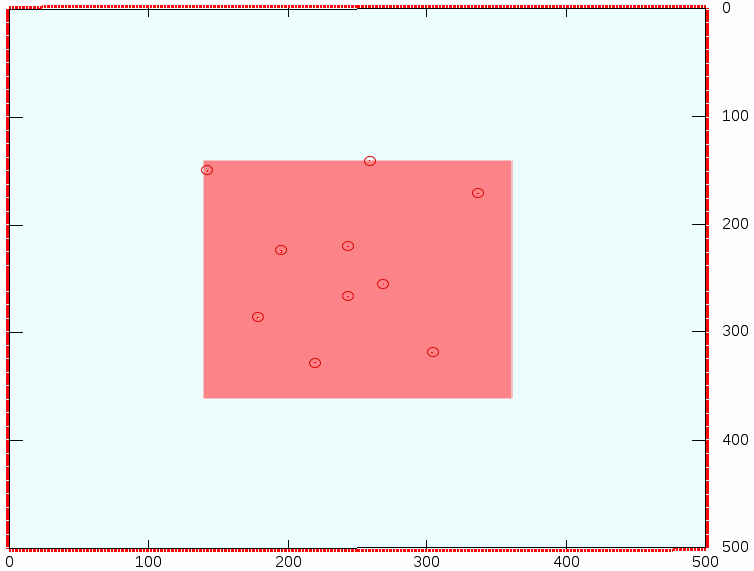
\includegraphics[width=0.48\hsize]{green/images/resultate/grfl/step0111.png}\vspace{1cm}\\
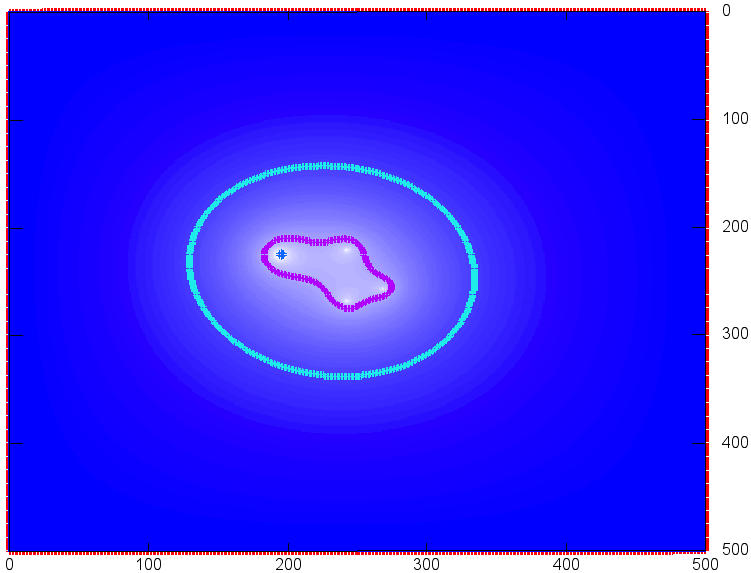
\includegraphics[width=0.48\hsize]{green/images/resultate/cp/step0057.png}
& 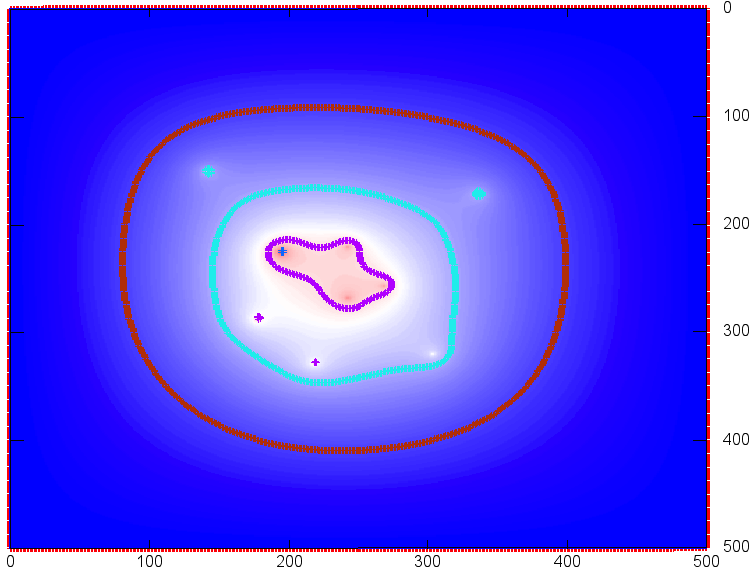
\includegraphics[width=0.48\hsize]{green/images/resultate/cp/step0111.png}\vspace{1cm}\\
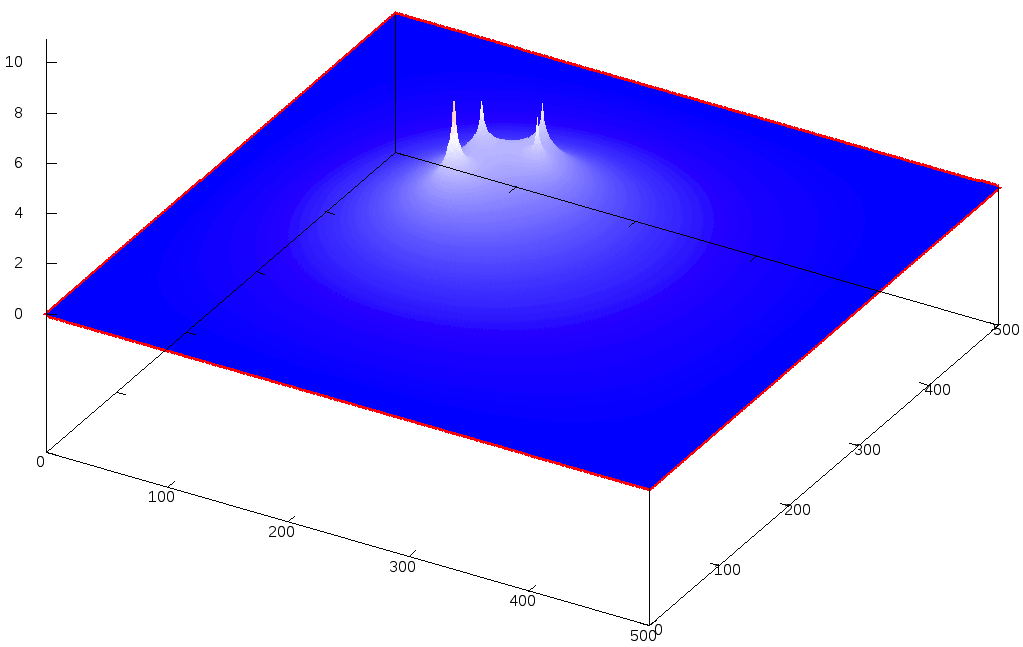
\includegraphics[width=0.48\hsize]{green/images/resultate/np/step0057.png}
& 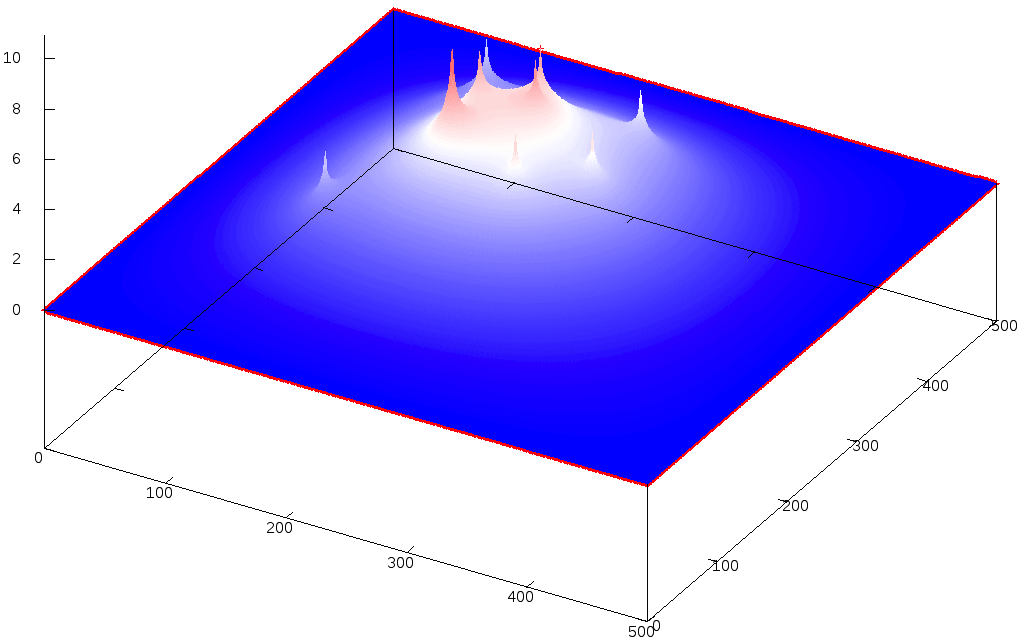
\includegraphics[width=0.48\hsize]{green/images/resultate/np/step0111.png}
\end{tabular}		
\caption{Visualisierung von Green's Function: Schritte 75 und 111 }
\end{figure}
	
\begin{figure}
\centering
\begin{tabular}{cc}
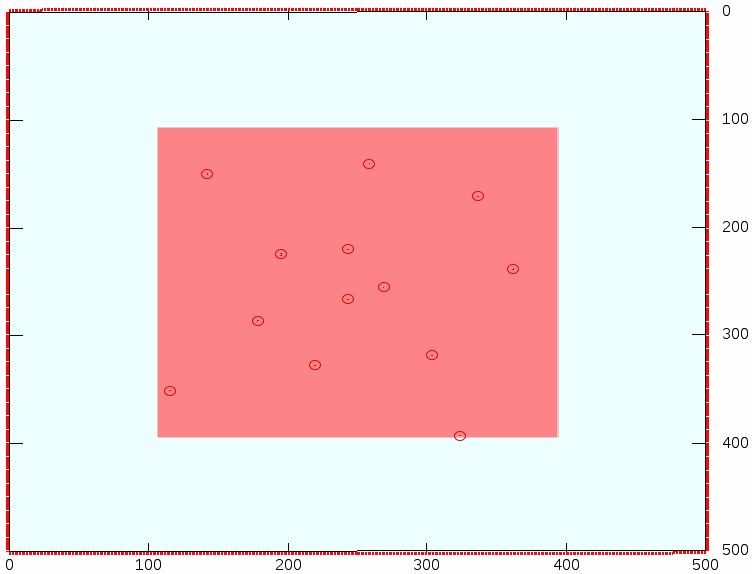
\includegraphics[width=0.48\hsize]{green/images/resultate/grfl/step0144.png}
& 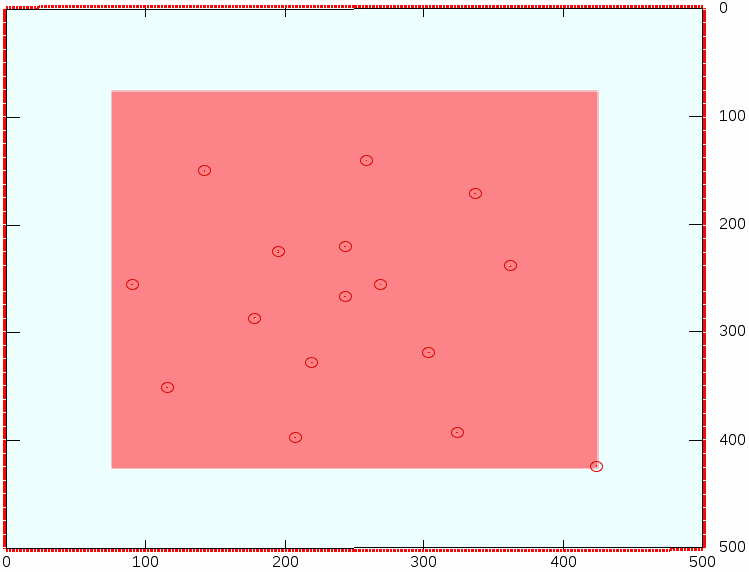
\includegraphics[width=0.48\hsize]{green/images/resultate/grfl/step0175.png}\vspace{1cm}\\
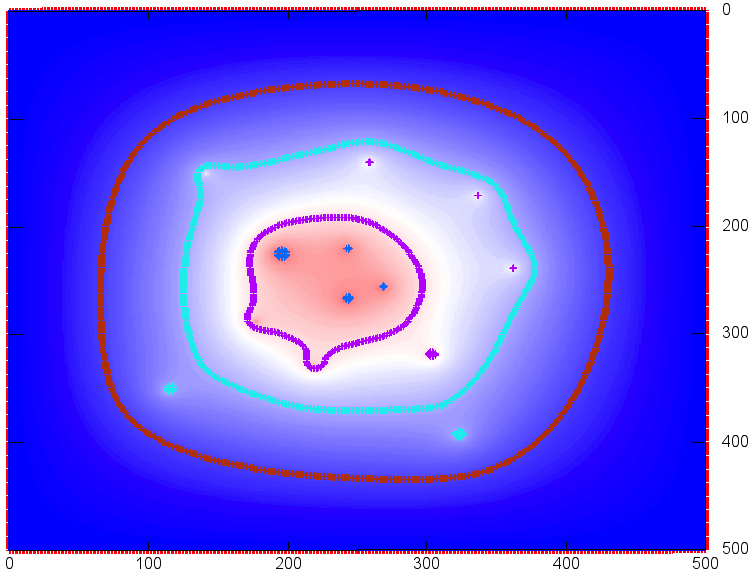
\includegraphics[width=0.48\hsize]{green/images/resultate/cp/step0144.png}
& 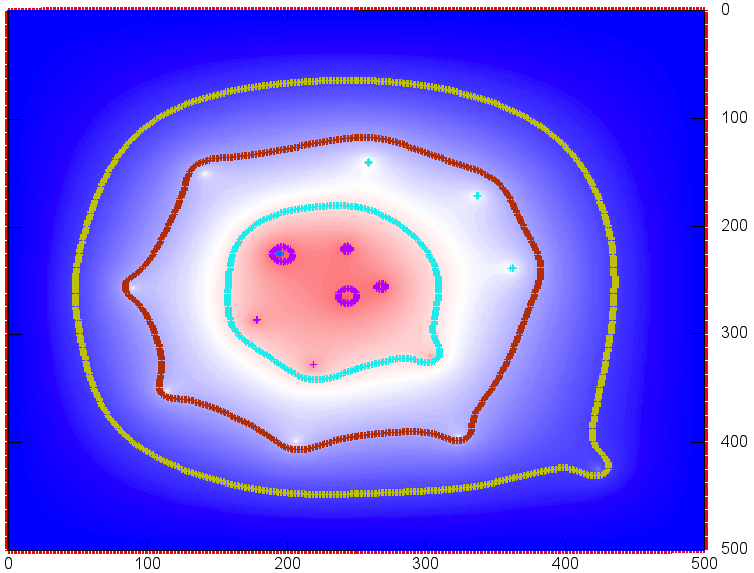
\includegraphics[width=0.48\hsize]{green/images/resultate/cp/step0175.png}\vspace{1cm}\\
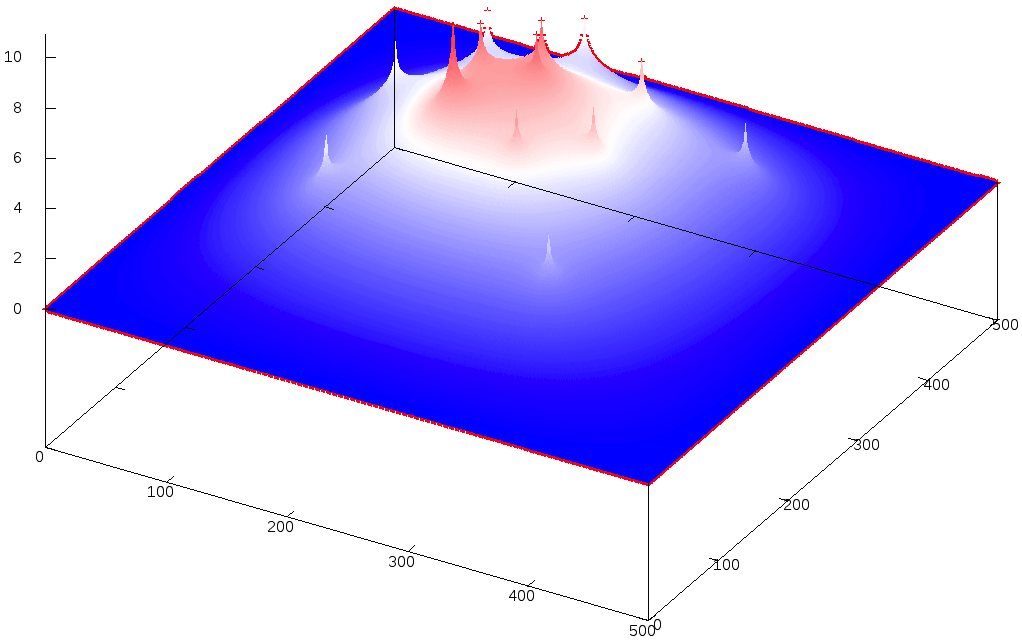
\includegraphics[width=0.48\hsize]{green/images/resultate/np/step0144.png}
& 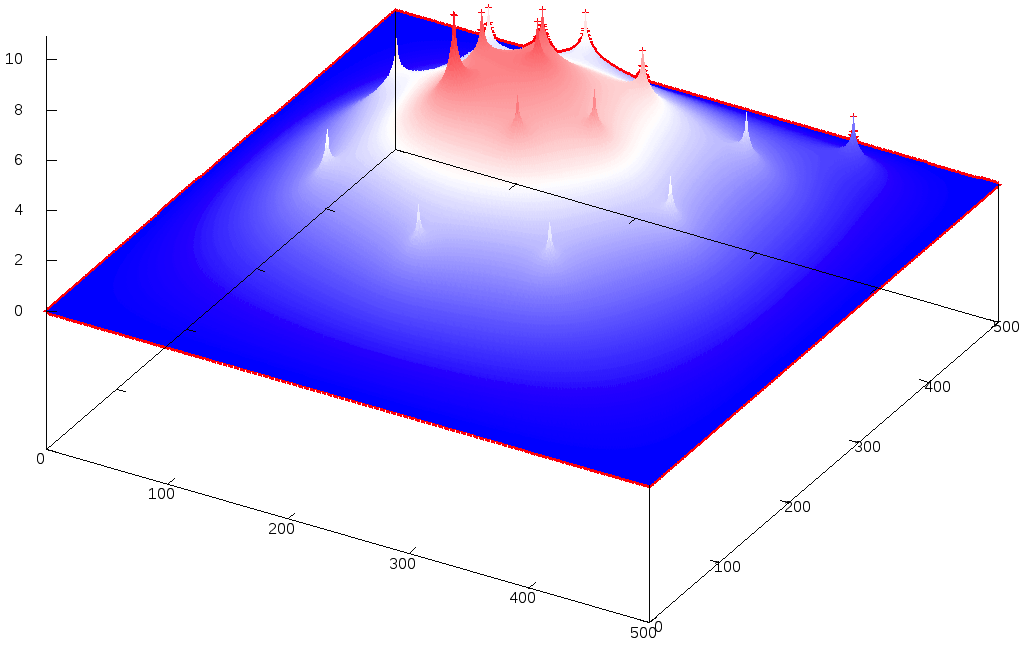
\includegraphics[width=0.48\hsize]{green/images/resultate/np/step0175.png}
\end{tabular}		
\caption{Visualisierung von Green's Function: Schritte 144 und 175 }
\end{figure}

\printbibliography[heading=subbibliography]
\end{refsection}
